%%%%%%%%%%%%%%%%%%%%%%%%%%%%%%%%%%%%%%%%%%%%
% https://github.com/martinhelso/uioposter %
%%%%%%%%%%%%%%%%%%%%%%%%%%%%%%%%%%%%%%%%%%%%
% Class options                            %
%%%%%%%%%%%%%%%%%%%%%%%%%%%%%%%%%%%%%%%%%%%%
% Orientation:                             %
% portrait (default), landscape            %
%                                          %
% Paper size:                              %
% a0paper (default), a1paper, a2paper,     %
% a3paper, a4paper, a5paper, a6paper       %
%                                          %
% Language:                                %
% english (default), norsk                 %
%%%%%%%%%%%%%%%%%%%%%%%%%%%%%%%%%%%%%%%%%%%%
\documentclass{uioposter}


\usepackage{lipsum}                                % Dummy text
\usepackage[figwidth = 0.98\linewidth]{todonotes}  % Dummy image (and more!)
\usepackage[absolute, overlay]{textpos}            % Figure placement
\setlength{\TPHorizModule}{\paperwidth}
\setlength{\TPVertModule}{\paperheight}


\title{Project \#1}
\author
{%
    AKA. 3 way Duel
    \and
    AKA. Source Duels
    \and
    AKA. Ninjason's unnamed project
}
%% Optional:
\institute
{
    3 Players
    \and
    5-10 minutes
    \and
    ages 10?+ idk
}
% Or:
%\institute{Contact information}


%% Remove footline:
%\setbeamertemplate{footline}{}


\begin{document}
\begin{frame}
\begin{columns}[onlytextwidth]


\begin{column}{0.5\textwidth - 1.5cm}

    \begin{block}{Introduction}
        \{project \#1\} is a small tactical game for 3 players, where every turn counts, balance attacking and defending, and utilizing every positional detail and sometimes a little teamwork to your advantage to claim victory
    \end{block}

    \begin{block}{Setup}
        \raggedright
        First set up your board as shown below and designate a corner for each player's 'Base' this should use a total of 25 hexes
        \begin{center}
            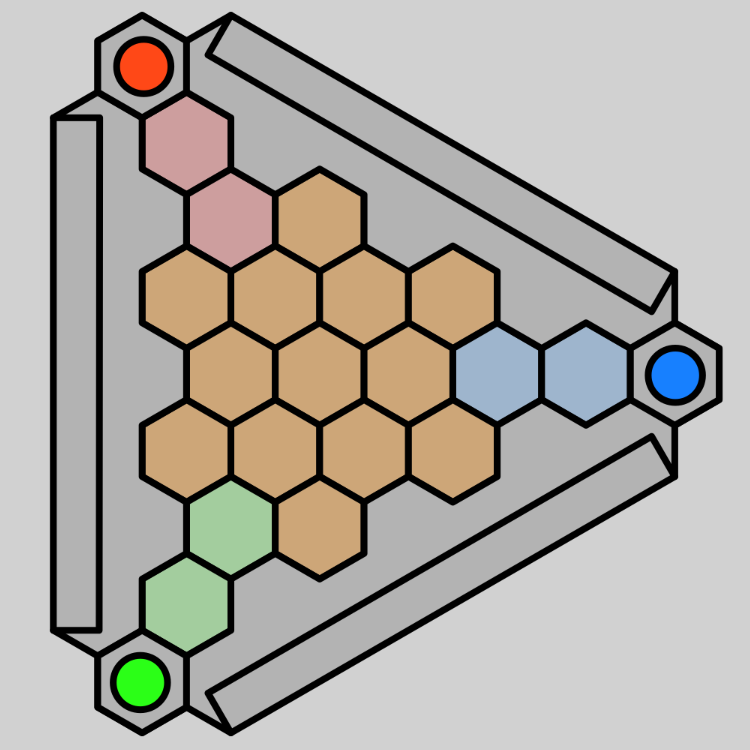
\includegraphics[]{Img/3DuelBoard.png}
        \end{center}
        each player chooses a character, and then place each of the players character and weapon in their corner, with their weapon in the corner space. choose a player to start, then begin!
    \end{block}

    \begin{block}{Winning}
        The goal of the game is to get a point from each of your opponents. you get a point by either knocking them out or entering their base.
    \end{block}

    \begin{alertblock}{Characters}
        All characters always have the basic move and jump ability, but how they attack will be determined by the character... for beginners I recommend starting with a game with all 3 players playing as "swords"
    \end{alertblock}

\end{column}

\begin{column}{0.5\textwidth - 1.5cm}

    \begin{block}{On your Turn}
        On your turn, you must make a move if possible, if no possible moves exist, your turn is skipped. most moves can be categorized in 2 ways, Attacks, and Movements. an attack does not move your character, but knocks out an opponent. you must successfully knock out an opponent to take an attack action, if an action moves your character, it does not have to successfully attack and can be considered a movement
    \end{block}

    \begin{block}{Getting knocked out}
        if you are knocked out, you are not out of the game, simply place your pieces back in your starting position, if there are already any pieces there, move them to the next closest valid space, if there are multiple options, the player getting moved has the choice
    \end{block}
    
    \begin{block}{Basic move}
        Move your character to any adjacent space
        then place your weapon in any space adjacent to your character.
        you may not place ether in a space already occupied by an opponent's character or weapon.
        you may move into the space containing your own weapon.
        you do not have to move your weapon as long as it is still in an adjacent space
    \end{block}

    \begin{block}{Jump}
        you may "jump" over your weapon, leaving it in the same position, but moving your character to the opposite side.
    \end{block}

    \begin{exampleblock}{Character: Sword}
        you may attack staying in the same spot, knocking out a player by placing your weapon in their space, you may "swing" your weapon upto 2 spaces, remaining adjacent to you. you may not move your weapon through an opponents weapon, or any "spaces" off the board, you may also attack using the jump ability, knocking out an opponent if they are where you land on a jump.
    \end{exampleblock}

    
\end{column}


\end{columns}


\begin{textblock}{0.5}(0.18, 0.93)
    \color{white}
    \sffamily
    \textbf{Compatible with the Source system}
    \\
    Designed by masterninjason.
    \\
    v0.1
\end{textblock}


\end{frame}
\end{document}
